\label{Schaltungslayout}

In Abbildung \ref{fig:Layout} ist das Schaltungslayout des Projektes zu sehen, welches wir mithilfe von Fritzing angefertigt haben. \\
Das \ac{LCD}-Display ist an sechs Pins mit dem Arduino verbunden. Zudem benötigt das \ac{LCD} eine Versorgungsspannung von ca. 5 Volt. Der Eingang V0 ist dabei über einen Widerstand auf Masse geschalten. Je nach Höhe des Widerstandes ändert sich der Kontrast des \ac{LCD}-Displays. \\
Darunter befindet sich in Abbildung \ref{fig:Layout} der CO2-Sensor CCS811, welcher über zwei Pins an den Arduino angeschlossen ist. Einen extra Anschluss an die Versorgungsspannung benötigt dieser nicht, da er die maximal benötigten $3.6$ Volt über den I$^2$C-Anschluss bekommt. \\
Unterhalb des Co2-Sensors ist das SD-Karten-Modul zu sehen, welches eine Versorgungsspannung von 5 Volt auf Masse benötigt. Die restlichen vier Anschlüsse sind mit den Pins 8 bis 11 am Arduino verbunden. \\
Zwei von den oben zu sehenden Taster dienen für die Menüauswahl auf dem \ac{LCD}-Display. Einer soll dabei für das Wechseln innerhalb des Menüs dienen, der andere ist für die Bestätigung der Auswahl zuständig. Damit die Schaltung auch ein- und ausgeschaltet werden kann, ohne die Versorgungsspannung zu kappen, haben wir einen dritten Taster eingebaut. Die Vorwiderstände aller Taster belaufen sich auf $2\kilo\ohm$. \\
Die vier LEDs sind, wie in den Anforderungen definiert, für die Visualisierung der Luftgüte zuständig. Dabei dienen die Farben Grün, Gelb und Rot für gute, mittlere und schlechte Luftgüte. Die blaue simuliert den angeschlossenen Fensterscheibenmotor. Für die Vorwiderstände der vier LEDs haben wir jeweils $330\ohm$ gewählt. \\

\begin{figure}[!hbt]
	\centering
	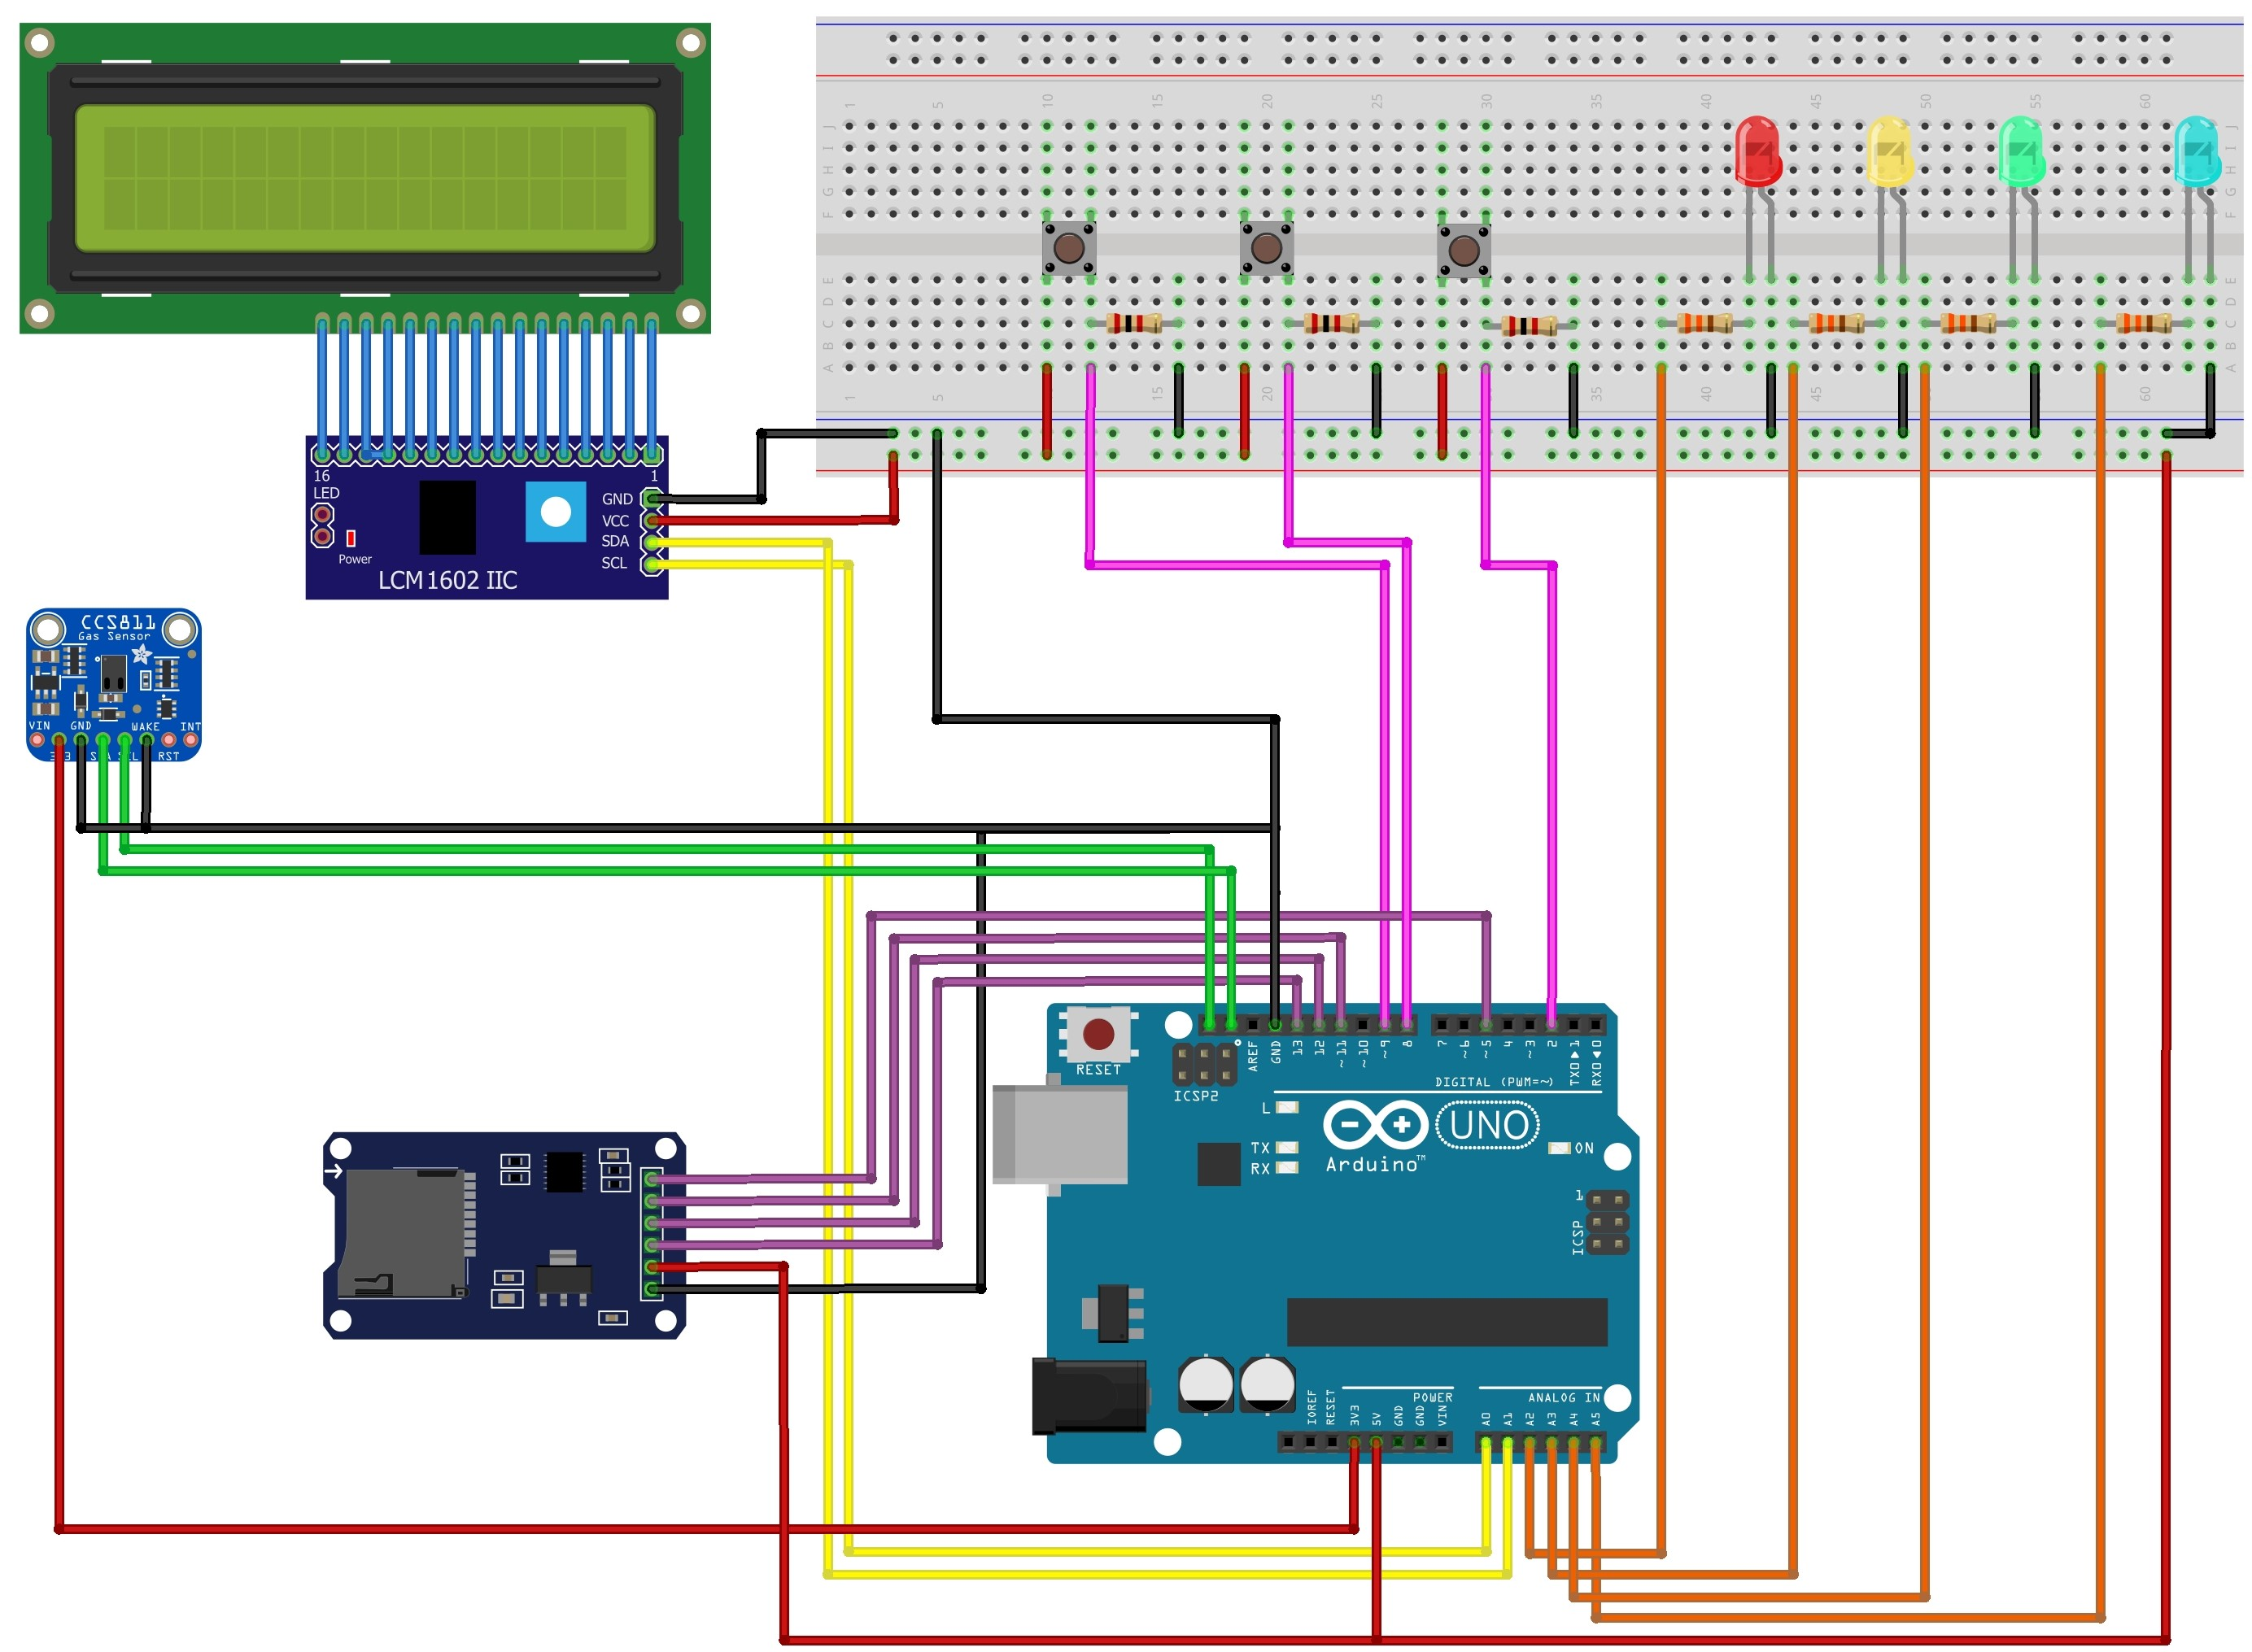
\includegraphics[width=0.9\linewidth]{Images/Layout_Steckplatine}
	\caption{Schaltungslayout vom 27.02.2020}
	\label{fig:Layout}
\end{figure}